\documentclass[11pt,a4paper]{article}
\usepackage[T1]{fontenc}
\usepackage[utf8]{inputenc}
\usepackage{lmodern}
\usepackage[margin=22mm,headheight=15pt,headsep=8mm,footskip=12mm]{geometry}
\usepackage{microtype}
\usepackage{xcolor}
\usepackage{amsmath}
\usepackage{booktabs,tabularx,array}
\usepackage{enumitem}
\usepackage{listings}
\usepackage{fancyhdr}
\usepackage{titlesec}
\usepackage{tikz}
\usetikzlibrary{arrows.meta,positioning}
\usepackage{hyperref}
\definecolor{ink}{HTML}{173642}
\definecolor{teal}{HTML}{007C83}
\definecolor{muted}{HTML}{52636B}
\definecolor{paperblue}{HTML}{F1F6F7}
\definecolor{rulegray}{HTML}{CFDDE0}
\hypersetup{colorlinks=true,linkcolor=teal,urlcolor=teal,pdftitle={Setting up a multi-agent research experiment in Codex},pdfauthor={Prepared with Codex},pdfsubject={Installation, agent files, review protocol, accounting and reproducibility}}
\urlstyle{same}
\pagestyle{fancy}
\fancyhf{}
\fancyhead[L]{\small\sffamily\color{muted}CODEX\quad /\quad RESEARCH SETUP GUIDE}
\fancyfoot[L]{\small\sffamily\color{muted}Practical handbook\quad\textbullet\quad 21 October 2026}
\fancyfoot[R]{\small\sffamily\color{muted}\thepage}
\renewcommand{\headrulewidth}{0.3pt}
\renewcommand{\footrulewidth}{0pt}
\setlength{\parindent}{0pt}
\setlength{\parskip}{6pt}
\setlength{\emergencystretch}{2em}
\setlist[itemize]{leftmargin=1.5em,itemsep=3pt,topsep=4pt,parsep=0pt}
\setlist[enumerate]{leftmargin=1.6em,itemsep=4pt,topsep=4pt,parsep=0pt}
\titleformat{\section}{\Large\bfseries\sffamily\color{ink}}{}{0pt}{}
\titleformat{\subsection}{\normalsize\bfseries\sffamily\color{teal}}{}{0pt}{}
\titlespacing*{\section}{0pt}{0pt}{10pt}
\titlespacing*{\subsection}{0pt}{10pt}{4pt}
\lstdefinestyle{guide}{basicstyle=\ttfamily\fontsize{8.7}{10.5}\selectfont,backgroundcolor=\color{paperblue},frame=single,rulecolor=\color{rulegray},framerule=0.3pt,framesep=6pt,xleftmargin=6pt,xrightmargin=6pt,breaklines=true,breakatwhitespace=false,columns=fullflexible,keepspaces=true,showstringspaces=false,upquote=true,aboveskip=8pt,belowskip=7pt,tabsize=2}
\lstset{style=guide}
\newcommand{\pathcode}[1]{\texttt{\small\detokenize{#1}}}
\newcommand{\step}[2]{\section*{#1\quad #2}}
\newcommand{\note}[2]{\par\smallskip\noindent\colorbox{paperblue}{\parbox{\dimexpr\linewidth-2\fboxsep\relax}{\textbf{#1}\ #2}}\par\smallskip}
\newcolumntype{Y}{>{\raggedright\arraybackslash}X}
\begin{document}

% PAGE 1
\thispagestyle{empty}
{\sffamily\small\color{teal}A PRACTICAL GUIDE\hfill 21 OCTOBER 2026}
\vspace{15mm}

{\sffamily\bfseries\fontsize{29}{34}\selectfont\color{ink}Setting up a multi-agent\\research experiment\\in Codex\par}
\vspace{5mm}
{\Large\color{muted}From installation to an auditable research record\par}
\vspace{8mm}

This guide explains how to organise a mathematical research experiment with a coordinator, independent investigators and fresh reviewers. It includes project files, configuration examples, launch prompts, submission limits and token-accounting rules.

The worked architecture comes from the reciprocal-simplex experiment in the \href{https://github.com/MathisRost/agentic-ai-math/tree/main/experiments/reciprocal-simplex-astra6}{\texttt{agentic-ai-math} repository}. It is a reusable research protocol: replace the mathematical statement and approach assignments to study another problem.

\subsection*{What you will build}
\begin{center}
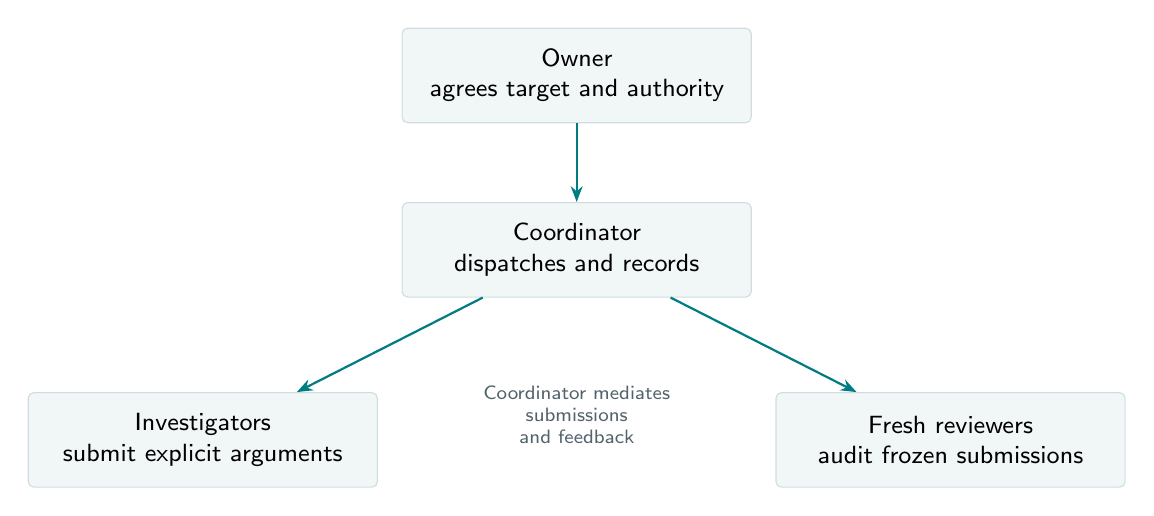
\begin{tikzpicture}[font=\small\sffamily,node distance=10mm,box/.style={draw=rulegray,fill=paperblue,rounded corners=2pt,align=center,minimum height=12mm,text width=42mm},arr/.style={-{Stealth[length=2mm]},draw=teal,thick}]
\node[box] (owner) {Owner\\agrees target and authority};
\node[box,below=of owner] (coord) {Coordinator\\dispatches and records};
\node[box,below left=12mm and 3mm of coord] (invest) {Investigators\\submit explicit arguments};
\node[box,below right=12mm and 3mm of coord] (review) {Fresh reviewers\\audit frozen submissions};
\draw[arr] (owner)--(coord);
\draw[arr] (coord)--(invest);
\draw[arr] (coord)--(review);
\node[below=10mm of coord,align=center,text width=27mm,font=\scriptsize\sffamily,color=muted] {Coordinator mediates\\submissions and feedback};
\end{tikzpicture}
\end{center}

\subsection*{How to use this guide}
Follow the steps in order. Prepare the files first, run a technical preflight, then explicitly launch research. The configuration examples use \texttt{gpt-6-astra} with \texttt{xhigh}, as in the worked experiment; availability must be checked in your own account.

\note{Scope.}{This is a setup and documentation guide. Agent review provides a structured audit, not formal proof certification. Saved records should contain explicit proofs and concise reasoning summaries, not private chain-of-thought.}

\vfill
{\small\color{muted}Software instructions were checked for the accompanying guide on 21 October 2026. Interfaces and configuration support can change; official documentation and the archived example are linked on the final page.}
\newpage

% PAGE 2
\step{1--3}{Install Codex and create the project}
\subsection*{1. Download, install and sign in}
Use the \href{https://learn.chatgpt.com/docs/app}{official desktop installation page}. The documentation checked for this guide calls the installer the ChatGPT desktop app; select \textbf{Codex} inside it. Install the app and sign in with your ChatGPT account.

Open a \textbf{local project} so the coordinator can read and write the experiment files. An API key, Python and the command-line version of Codex are not required merely to coordinate the agents. Computation and PDF production may require additional tools. See the \href{https://learn.chatgpt.com/docs/quickstart}{official quickstart} for the current interface.

\subsection*{2. Create a clean folder}
Create a folder such as \pathcode{Documents/mathematical-research/experiment-01}. Open it in Codex and start a chat there. That chat is the coordinator. Keep previous results outside the new project when independence from earlier solutions matters.

You can create the files yourself or ask Codex to prepare them. Start with this instruction:
\begin{quote}
Prepare the experiment files only. Do not launch research agents or investigate the mathematical problem yet.
\end{quote}

\subsection*{3. Use a predictable directory structure}
\begin{lstlisting}
experiment-01/
  AGENTS.md
  START.md
  workflow.json
  .codex/
    config.toml
    agents/
      nonexistence_1.toml
      nonexistence_2.toml
      proof_1.toml                 # also proof_2, proof_3, proof_4
      reviewer.toml
      literature.toml
  common/problem_statement.md
  instructions/
    coordinator.md
    nonexistence.md
    proof.md
    reviewer.md
    accounting.md
  approaches/                     # one assignment per approach
  starting_information/           # construction-only prior leads
  sources/                        # supplied papers and source index
  templates/                      # submissions, reviews, accounting
  runs/                           # all experiment outputs
\end{lstlisting}

\note{Two kinds of file.}{\pathcode{.codex/config.toml} and the agent TOML files configure Codex. \pathcode{START.md}, \pathcode{workflow.json} and the other research documents are conventions you introduce. The coordinator follows them because you instruct it to do so; the JSON file is not a built-in workflow engine.}
\newpage

% PAGE 3
\step{4--5}{Fix the target and the project rules}
\subsection*{4. Write the exact mathematical problem}
Save the initial statement as \pathcode{common/problem_statement.md} and label it \textbf{S0}. Define the objects, assumptions, quantifiers and conclusion. Specify which parameters are prescribed and which may be chosen.
\begin{lstlisting}
# Problem statement - S0

## Objects and notation
Define all objects and symbols.

## Assumptions and quantifiers
List every permitted assumption. State which parameters are fixed.

## Required conclusion
State the exact theorem or construction sought.

## Success criterion
A complete argument satisfying every requirement of S0.

## Partial results
Identify results that do not meet the full target: approximations,
extra hypotheses, restricted subclasses or numerical evidence.
\end{lstlisting}

For example, an exact identity for product densities must not quietly become an asymptotic statement or an identity for connected densities. A prescribed positive intensity must not become a freely chosen small intensity.

\subsection*{5. Put persistent rules in AGENTS.md}
Codex reads \pathcode{AGENTS.md} as project instructions. Personal or parent-directory instructions may also apply; inspect the effective rules before starting. See the \href{https://learn.chatgpt.com/docs/agent-configuration/agents-md}{official documentation}.
\begin{lstlisting}
# Research experiment rules

1. Do not launch research until the owner explicitly requests START.
2. The initial target is common/problem_statement.md, version S0.
3. Verify the agreed model and effort before research; no silent fallback.
4. Only the coordinator dispatches agents.
5. Use fresh contexts and explicit input packets for independent work.
6. Begin with two independent non-existence investigations.
7. Every frozen submission receives a fresh independent review.
8. A class-specific obstruction does not disprove the general target.
9. Each construction approach has four substantive submissions total.
10. After three unsuccessful reviewed submissions, an investigator may
    request a precise target amendment. Explicit owner approval is
    required. Attempt counts never reset automatically.
11. Save all outputs under runs/<run_id>/; preserve submitted versions.
12. Record exposed usage counters; unavailable means NR, not zero.
13. Save explicit proofs and concise reasoning and decision summaries.
14. Follow workflow.json and instructions/coordinator.md.
\end{lstlisting}

\textbf{Decide revision authority in advance.} State whether a reviewed general obstruction permits a coordinator-led restriction or whether every statement change requires owner approval. Record the logical necessity separately from the choice of repair. An obstruction assuming finite moments does not by itself restrict a target without that assumption.
\newpage

% PAGE 4
\step{6--7}{Configure the model and an investigator}
\subsection*{6. Create .codex/config.toml}
The worked experiment used the following project configuration:
\begin{lstlisting}
model = "gpt-6-astra"
model_reasoning_effort = "xhigh"

[agents]
enabled = true
max_concurrent_threads_per_session = 3
default_subagent_model = "gpt-6-astra"
default_subagent_reasoning_effort = "xhigh"
\end{lstlisting}

The concurrency value permits up to three spawned-agent threads in addition to the coordinator. It does not limit the number of agents used over the entire experiment. Schedule later investigators and fresh reviews as capacity becomes available.

Project configuration loads only for trusted projects. Use the normal trust flow for a folder you control. A saved model name neither proves account access nor necessarily switches a running coordinator. Start a fresh chat after setup and verify the actual settings. See \href{https://learn.chatgpt.com/docs/config-file/config-basic}{configuration basics} and the \href{https://learn.chatgpt.com/docs/config-file/config-reference}{configuration reference}.

\subsection*{7. Define specialised agent roles}
Create one TOML file per role in \pathcode{.codex/agents/}. The essential fields are \texttt{name}, \texttt{description} and \texttt{developer\_instructions}. Here is \pathcode{proof_1.toml}:
\begin{lstlisting}
name = "proof_1"
description = "Develop an exact construction using approach 1."
model = "gpt-6-astra"
model_reasoning_effort = "xhigh"

developer_instructions = """
You are an independent construction investigator. Do not delegate.

Before mathematical work, require a coordinator packet containing:
- the active statement path, version and hash;
- the permitted inputs and your approach instructions;
- your submission number and assigned output paths.

Read the assigned project, proof and accounting instructions.
Do not read other construction tracks or previous experiments.
Prove every claimed property. Identify gaps and extra assumptions.
A partial result is not an exact-target success.

You have four substantive submissions total.
A target amendment does not reset this count.
Write only to assigned paths. Save an explicit proof and a concise
reasoning summary. Report unavailable usage fields as NR.
"""
\end{lstlisting}

\note{Configuration does not launch research.}{Agent files define available roles. Explicit delegation requests or applicable project instructions cause the coordinator to use them. See the \href{https://learn.chatgpt.com/docs/agent-configuration/subagents}{custom-agent documentation}.}
\newpage

% PAGE 5
\step{7 continued}{Define reviewers and the remaining roles}
A reviewer receives a frozen submission and the exact target it claims to meet. Create \pathcode{.codex/agents/reviewer.toml}:
\begin{lstlisting}
name = "reviewer"
description = "Independently audit a frozen mathematical submission."
model = "gpt-6-astra"
model_reasoning_effort = "xhigh"

developer_instructions = """
Audit only the assigned frozen statement, submission and sources.
Do not delegate.

Check definitions, quantifiers, hidden assumptions, limiting
arguments, integrability and every claimed identity.

Distinguish a proved exact result, partial progress, an invalid
argument and an unresolved obligation. Explain your verdict.
Do not silently repair the proof or weaken the target.
Write the review to the assigned path.
"""
\end{lstlisting}

\subsection*{Role assignments}
Use the same file pattern for the other roles. Put detailed mathematical assignments in the corresponding instruction and approach files.

\renewcommand{\arraystretch}{1.22}
\begin{tabularx}{\linewidth}{@{}p{36mm}Y@{}}
\toprule
\textbf{Role} & \textbf{Responsibility}\\
\midrule
Coordinator & Main chat; dispatches, records decisions, updates statements and ledgers.\\
\texttt{nonexistence\_1} & Investigates general obstructions without construction seeds.\\
\texttt{nonexistence\_2} & Independently investigates obstructions from another assigned perspective.\\
\texttt{proof\_1}--\texttt{proof\_4} & Each pursues its own construction approach.\\
\texttt{reviewer} & Audits one frozen submission in a fresh context.\\
\texttt{literature} & Checks precise mathematical claims against primary sources.\\
Optional \texttt{coder} & Performs specific reproducible checks requested by the coordinator.\\
\bottomrule
\end{tabularx}

\subsection*{Fresh contexts are part of the design}
A role definition can be reused, but each independent review should start in a fresh agent context. Do not copy the author's entire conversation or private work notes into the reviewer. Send the explicit proof and assigned evidence.

Similarly, the two obstruction investigators should not receive each other's arguments while developing their submissions. Construction agents may receive the same frozen starting-information packet after the obstruction phase. Label prior proofs as leads to verify, not accepted conclusions of the new experiment.

\note{Optional skills.}{A reusable review procedure can be packaged as \pathcode{.agents/skills/<name>/SKILL.md}. A skill defines a procedure; an agent file defines a role. Start with ordinary instruction files if that is simpler. See the \href{https://learn.chatgpt.com/docs/build-skills}{skills documentation}.}
\newpage

% PAGE 6
\step{8}{Write the workflow and coordinator instructions}
Save the experiment's stages and limits in \pathcode{workflow.json}:
\begin{lstlisting}
{
  "initial_statement": "S0",
  "phases": [
    "preflight",
    "independent_obstructions",
    "obstruction_reviews",
    "target_decision",
    "independent_constructions",
    "submission_reviews",
    "final_synthesis"
  ],
  "construction_submission_limit": 4,
  "amendment_request_after_reviewed_failures": 3,
  "amendments_reset_attempt_count": false,
  "fresh_review_context": true,
  "only_coordinator_dispatches": true,
  "accounting_preflight_required": true
}
\end{lstlisting}

Explain its execution in \pathcode{instructions/coordinator.md}:
\begin{enumerate}
\item Create one run directory. Freeze the intended inputs, initial statement and configuration with hashes.
\item Complete the model-access and accounting preflight before mathematical research.
\item Dispatch two independent obstruction investigators. Freeze each submission and commission a fresh review.
\item Decide the active target under the agreed revision authority. Record exactly what an obstruction proves and which repair has been chosen.
\item Give each construction investigator the approved target and permitted inputs. Keep ideas from separate tracks separate until synthesis.
\item Freeze each substantive submission, update its attempt count and obtain a fresh review. Send the investigator its own review for a permitted repair.
\item After three reviewed failures, allow an optional precise amendment request. Until the owner approves, retain the current target and attempt count.
\item After four failed submissions, mark that approach unsuccessful. Do not infer that the theorem is false.
\item Finish with an independent synthesis and a report of accepted results, failures, unresolved obligations and accounting coverage.
\end{enumerate}

\subsection*{Keep decisions auditable}
For every target change, save the old and new statements, the supporting reviews, a precise explanation, its authority and the owner's response when required. Broadcast each adopted version and its evidence to every role, including resumed agents.

\note{Separate responsibilities.}{The coordinator owns shared targets and ledgers. Investigators own assigned submission files. Reviewers own assigned review files. An author must not overwrite a frozen submission after a reviewer has started reading it.}
\newpage

% PAGE 7
\step{9--10}{Control inputs and standardise submissions}
\subsection*{9. Create an explicit dispatch packet}
A packet states exactly what an agent is to read and produce. For example:
\begin{lstlisting}
# Dispatch: proof_1, submission 1 of 4

Active statement: statements/S1.md
Statement SHA-256: <insert actual hash>

Permitted inputs:
- inputs/AGENTS.md
- inputs/instructions/proof.md
- inputs/approaches/01.md
- inputs/starting_information/<assigned files>

Assigned outputs:
- tracks/proof_1/submissions/v01.md
- tracks/proof_1/summaries/v01.md

Do not read other construction tracks, earlier experiments,
unassigned chats or private notes.

Required result:
An explicit construction satisfying S1, or a precise account of
which obligations remain unresolved.
\end{lstlisting}

Replace placeholders before dispatch. For the initial non-existence agents, omit construction seeds. References should resolve to the frozen run inputs rather than mutable originals.

These read restrictions establish \textbf{procedural independence}. They are not operating-system isolation. Agents sharing a workspace may technically be able to read other files. If strict isolation is required, use separate environments with enforced access restrictions.

\subsection*{10. Use submission and review templates}
\begin{lstlisting}
# Submission metadata
Role, target version/hash, submission number and timestamps.

# Exact claim
The precise result claimed.

# Construction or obstruction
Definitions and a complete explicit argument.

# Verification
Check each target requirement separately.

# Unresolved obligations
List gaps and extra assumptions.

# Reasoning summary and sources
Summarise the approach and decisive checks; identify source results.
\end{lstlisting}

A review should identify the statement and submission hashes, state its verdict, and justify it through mathematical checks. Include negative findings and unresolved obligations. ``Looks correct'' is not an adequate review. Numerical evidence belongs in a separate section and is not a proof of an exact identity.
\newpage

% PAGE 8
\step{11}{Plan token, cost and runtime accounting}
Put the accounting rules in \pathcode{instructions/accounting.md}. Check what the runtime actually exposes before the research starts. A percentage of subscription usage is not a per-agent token count.

\begin{tabularx}{\linewidth}{@{}p{47mm}Y@{}}
\toprule
\textbf{Record} & \textbf{Purpose}\\
\midrule
Run, agent and turn IDs & Identify whose work is being measured.\\
Role, target and attempt & Connect usage to the experiment.\\
Requested/observed model & Separate configuration from execution evidence.\\
Start and end timestamps & Establish runtime boundaries in UTC.\\
Input, cached input, output & Preserve exposed numeric counters and semantics.\\
Reasoning tokens & Record separately when exposed; check overlap with output.\\
Source and coverage & Identify exact, partial or unavailable measurements.\\
Cost assumptions & Record prices, model, tier, date and relevant context band.\\
\bottomrule
\end{tabularx}

\subsection*{Rules that prevent misleading totals}
\begin{itemize}
\item Unknown measurements are \texttt{NR} in tables and \texttt{null} in JSON, never zero.
\item For cumulative counters, use valid differences between checkpoints. Do not sum snapshots.
\item Establish whether coordinator totals include child-agent usage before aggregating them.
\item Do not add cached input again if it is already included in input tokens. Do not add reasoning tokens again if they are included in output.
\item Record the observed service setting, including Fast where exposed. Do not infer it from response speed.
\item Keep setup, technical preflight, research and later documentation usage distinct.
\item Read only authorised session metadata. Do not collect private reasoning, credentials or unrelated chats to reconstruct usage.
\end{itemize}

\subsection*{Cost is a separate calculation}
If $I$ is total input, $I_c$ its cached subset and $O$ output, and the applicable prices per million tokens are known, a simple API-equivalent estimate is
\[
C_{\mathrm{estimate}}=
\frac{(I-I_c)p_{\mathrm{input}}+I_c p_{\mathrm{cached}}+O p_{\mathrm{output}}}{10^6}.
\]
Use this only when the counter definitions and pricing categories support it. Account separately for other applicable fees or categories. Freeze the official price source and retrieval date. A subscription session's estimated API-equivalent cost is not its actual charge.

\subsection*{Runtime also needs a definition}
Record per-agent elapsed time and the overall run's start and end. Summed agent runtime can exceed elapsed experiment time because agents run in parallel. Label both quantities.

\note{Accounting gate.}{If exact per-agent telemetry is unavailable, tell the owner before research and obtain a decision on proceeding with \texttt{NR} fields or labelled estimates. Do not silently switch to a paid API workflow to obtain counters.}
\newpage

% PAGE 9
\step{12}{Validate the setup before doing research}
Start a fresh coordinator chat after creating the configuration and role files. Run a technical check to make sure the intended roles, inputs, model settings and accounting mechanism work.

\subsection*{Copyable preflight prompt}
\begin{lstlisting}
Perform setup validation only. Do not investigate the mathematical
problem.

Read AGENTS.md, workflow.json and the coordinator and accounting
instructions. Check that every referenced file exists and that the
custom roles are available. Verify the actual coordinator model
and reasoning effort using available runtime evidence.

Create a prepared run directory and freeze the intended inputs.
Dispatch nonexistence_1 and nonexistence_2 in fresh contexts for a
technical check only. They must confirm their assigned roles,
permitted inputs, output paths and available model and usage
evidence. They must do no mathematical research.

Save accounting_capability.json. Distinguish verified fields from
unavailable fields. Report any missing capability before research
starts. These checks consume tokens but do not count as mathematical
submissions. Stop after preflight.
\end{lstlisting}

\subsection*{What a successful preflight establishes}
\begin{enumerate}
\item All referenced instructions, approach files and source documents exist.
\item The coordinator can use the intended custom roles.
\item The requested model and effort have execution evidence, or the absence of verification is explicitly reported.
\item The accounting report identifies available fields, counter semantics and unresolved aggregation questions.
\item Each agent can write to its assigned output location.
\item The prepared run has a stable identifier and frozen inputs.
\end{enumerate}

If a check fails, repair the setup and repeat the affected technical check. Do not label technical retries as mathematical submissions. Keep their usage in the preparation or preflight records.

\subsection*{A useful run directory}
\begin{lstlisting}
runs/<run_id>/
  inputs/                         # frozen setup and source additions
  statements/                     # S0, S1, ...; never overwrite
  packets/                        # input/output assignments
  tracks/<role>/submissions/      # v01, v02, v03, v04
  reviews/<role>_v01/             # fresh review of one version
  attempt_ledger.json
  decisions.md
  accounting_capability.json
  agent_accounting.jsonl
  hashes.json
  final_report.md
\end{lstlisting}
\newpage

% PAGE 10
\step{13--14}{Launch, monitor and close the experiment}
\subsection*{13. Start only after the preflight decision}
Write the launch instructions into \pathcode{START.md}. State the target, workflow, accounting gate, stopping rules and any owner decisions. Then explicitly launch with:
\begin{lstlisting}
Start the research experiment by reading START.md. Continue in the
prepared run directory and follow AGENTS.md, workflow.json and the
coordinator instructions.

Begin with frozen S0 and two independent non-existence agents.
Obtain fresh reviews before adopting an obstruction or restriction.

Allow four substantive submissions per construction approach.
After three unsuccessful reviewed submissions, an investigator may
request a precise owner-approved statement change. Do not adopt it
without approval or reset the attempt count.

Preserve frozen submissions, reviews, concise reasoning summaries,
decision records and per-agent usage records.
\end{lstlisting}

\subsection*{14. Monitor records, not just conversational updates}
Ask for compact status tied to saved statements, reviews and ledgers. A fictional example is:
\begin{lstlisting}
Active target: S1
proof_1: submission 2/4, under review
proof_2: ended at 1/4 after an accepted class obstruction
proof_3: submission 3/4, repair pending
proof_4: submission 2/4, exact-target claim under review
Owner decisions pending: none
Accounting coverage: <measured coverage and missing fields>
\end{lstlisting}

Preserve failed submissions. A repair receives a new version and review; it does not replace the earlier files. A class-specific obstruction may end that class's track under the agreed rules, but it cannot establish non-existence for the general target.

\subsection*{Close with an independent synthesis}
The final reviewer checks the exact accepted claim against the active statement and records remaining obligations. At this stage the coordinator may compare independent tracks and assemble the final report.

The deliverable should contain the frozen setup, all statement versions, dispatch packets, submissions, reviews, attempt ledger, decision history, source records and accounting data. Explain the architecture, chronology, accepted result, unsuccessful approaches and practical limitations.

\note{What hashes establish.}{Hashes identify the exact file version that was submitted or reviewed. They do not establish mathematical correctness. The record should make a later human audit possible.}
\newpage

% PAGE 11
\section*{A shortcut for preparing the files}
Once you understand the structure, you can ask Codex to create the scaffold instead of typing every file. Use this prompt in a new project, then inspect the generated files before preflight.

\begin{lstlisting}
Prepare, but do not start, a multi-agent mathematical research
experiment in this folder.

Create AGENTS.md, START.md, workflow.json, .codex/config.toml,
.codex/agents/*.toml, common/problem_statement.md, the role and
accounting instructions, approach assignments and output templates.

The exact target is:
[PASTE THE FULL MATHEMATICAL STATEMENT HERE]

Use the following agreed model and reasoning effort:
[MODEL AND EFFORT]
Do not silently substitute if unavailable.

The coordinator is this chat. Only it dispatches agents.
Begin with two independent non-existence investigators. Then use
four independent construction approaches with assigned methods.
Every frozen submission receives a fresh independent review.

Allow four substantive submissions per construction approach.
After three unsuccessful reviewed submissions, an investigator may
request a precise statement amendment. Only explicit owner approval
authorises that amendment. Never reset attempt counts automatically.

Write an explicit rule for the authority to revise the target after
a reviewed general obstruction. Keep class-specific failures and
obstructions with additional moment assumptions correctly scoped.

Use fresh contexts, explicit permitted-input packets and assigned
output paths. Do not share new construction ideas between tracks.
Store all run outputs in runs/<run_id>/. Preserve frozen versions
and hashes. Save explicit proofs and concise reasoning summaries.

Require an accounting preflight. Record measured usage per agent
and turn when exposed, NR otherwise. Separate estimates from
charges, and elapsed experiment time from summed agent runtime.

Check consistency and list any missing decisions or files.
Do not dispatch agents or investigate the mathematics yet.
\end{lstlisting}

\subsection*{Before pressing START}
\begin{itemize}
\item Replace every placeholder in the target, model settings and approach assignments.
\item Check that the rules in \pathcode{AGENTS.md}, the workflow and role files agree.
\item Confirm that the initial investigators cannot accidentally encounter prior results in their assigned packets.
\item Complete preflight and resolve model or accounting limitations.
\item Confirm the statement-change authority and the four-submission ledger.
\end{itemize}

The preparation prompt is a convenience. The reviewed setup files and the preflight record are what define the experiment.
\newpage

% PAGE 12
\section*{Documentation and worked example}
\subsection*{Official product documentation}
These links support the software setup. The research protocol, submission limits and independence rules are choices of this experiment.

\begin{enumerate}[label=\arabic*.]
\item \href{https://learn.chatgpt.com/docs/app}{Desktop app installation}\\
\url{https://learn.chatgpt.com/docs/app}
\item \href{https://learn.chatgpt.com/docs/quickstart}{Quickstart}\\
\url{https://learn.chatgpt.com/docs/quickstart}
\item \href{https://learn.chatgpt.com/docs/config-file/config-basic}{Configuration basics}\\
\url{https://learn.chatgpt.com/docs/config-file/config-basic}
\item \href{https://learn.chatgpt.com/docs/config-file/config-reference}{Configuration reference}\\
\url{https://learn.chatgpt.com/docs/config-file/config-reference}
\item \href{https://learn.chatgpt.com/docs/agent-configuration/subagents}{Subagents and custom agent definitions}\\
\url{https://learn.chatgpt.com/docs/agent-configuration/subagents}
\item \href{https://learn.chatgpt.com/docs/agent-configuration/agents-md}{Project instructions with AGENTS.md}\\
\url{https://learn.chatgpt.com/docs/agent-configuration/agents-md}
\item \href{https://learn.chatgpt.com/docs/build-skills}{Reusable skills}\\
\url{https://learn.chatgpt.com/docs/build-skills}
\end{enumerate}

\subsection*{The reciprocal-simplex experiment}
The \href{https://github.com/MathisRost/agentic-ai-math/tree/main/experiments/reciprocal-simplex-astra6}{public experiment folder} contains the research report, accounting and archived evidence. The \href{https://github.com/MathisRost/agentic-ai-math/tree/9593db57d32ed993a645f72159ea8f002b300049/experiments/reciprocal-simplex-astra6/archive/inputs}{frozen setup inputs} provide the worked example for this guide.

\begin{tabularx}{\linewidth}{@{}p{42mm}Y@{}}
\toprule
\textbf{Archive location} & \textbf{What to inspect}\\
\midrule
\pathcode{.codex/} & Model configuration and custom agent definitions.\\
\pathcode{AGENTS.md} & Persistent experimental rules.\\
\pathcode{START.md} & Original launch instructions.\\
\pathcode{workflow.json} & Stages, roles and submission policy.\\
\pathcode{instructions/} & Coordinator, investigator, review and accounting procedures.\\
\pathcode{common/} & The original exact mathematical target.\\
\pathcode{approaches/} & Assigned construction methods.\\
\pathcode{templates/} & Structured record formats.\\
\bottomrule
\end{tabularx}

\subsection*{Reusing the archive}
Copy only the intended setup material into a new project. Include the hidden \pathcode{.codex/} directory. Replace the mathematical target and approach assignments, check all paths, and provide your own required sources or skills. Personal skill bodies and copied third-party papers are omitted from the public archive.

Do not use the completed results as undisclosed input to a supposedly independent investigation. Keep the old experiment intact, create a new run, and repeat the technical preflight.

\vfill
{\small\color{muted}Prepared as a standalone guide from the documented experiment and the accompanying setup instructions. The editable LaTeX source is supplied with the PDF.}
\end{document}
